\rewrite{Aspecto não estacionário dos conjuntos: Aprendizado baseado em janelas (mais recente = mais importante, menos recente = menos importante) vs detecção de desvios de conceito}

\section{Desvios de Conceito} \label{chConceitos:FD:Desvios}

Na maioria das aplicações do mundo real, os dados são coletados durante um período de tempo. Para longos períodos, é plausível considerar que os exemplos não são independentes ou não possuem mesma distribuição. Em domínios complexos, é provável que a distribuição de classes mude de acordo com o tempo \cite{Gama2004}. Essas mudanças são conhecidas como desvios de conceito.

Desvios de conceito podem ser graduais, onde há uma transição suave entre as distribuições, ou abruptas, quando a distribuição muda repentinamente.

Abordagens que lidam com desvios de conceitos podem ser classificadas em duas categorias: aquelas que adaptam o modelo em intervalos regulares sem considerar que mudanças ocorreram e aquelas que primeiro detectam desvios de conceitos e, então, adaptam o modelo a essas mudanças. As abordagens da primeira categoria são aquelas que utilizam modelos de janelas temporais.

As estratégias que realizam a detecção de mudanças para posterior adaptação do modelo mantêm um monitoramento, realizado pela definição de indicadores baseados no modelo. Se um desvio é detectado durante o monitoramento, são aplicadas ações para a adaptação do modelo de aprendizado.

Os trabalhos \cite{Gama2004,Li2012,wu2012} trazem maiores informações sobre algumas estratégias de detecção de desvios de conceito.

\subsection*{Janelas Temporais} \label{chConceitos:FD:Janelas}

As janelas temporais são uma abordagem bastante utilizada para resolver a questão de conjuntos abertos (infinitos) como FD. Ao invés do considerar todo o conjunto de exemplos de um fluxo, são considerados subconjuntos de exemplos ao longo do tempo. Neste modelo, uma marca temporal está associada a cada exemplo, a fim de determinar se o exemplo é válido ou não, ou seja, se está dentro ou fora de uma determinada janela temporal.

Existem diferentes modelos de janelas que podem ser encontrados na literatura, os mais relevantes \cite{Zhu2002} são descritos a seguir:

\begin{description}
\item[Modelo \emph{Sliding Window}:] neste modelo apenas a informação mais recente do FD é armazenada em uma estrutura de dados (janela) cujo tamanho pode ser variável ou fixo. Esta é uma estrutura tipo \emph{First In, First Out}, que considera os exemplos de um determinado ponto no tempo atual até um ponto no passado. A \autoref{Fig:slidingWindow} traz um exemplo do modelo \emph{Sliding Window}, com comprimento fixo de janela, em três momentos do tempo ($t-2$, $t-1$ e $t$) representando o deslizamento da janela para que contenha os exemplos mais recentes no tempo mais atual $t$. Algoritmos que utilizam este modelo \cite{Ren2009} apenas atualizam os sumários estatísticos dos exemplos dentro da janela.

\item[Modelo \emph{Damped Window}:] também conhecido como \emph{time-fading}, este modelo considera a informação mais recente pela associação de pesos aos exemplos do FD \cite{Jiang2006}: exemplos mais recentes tem peso maior que exemplos mais antigos e o peso dos exemplos diminui de acordo com o tempo. Um exemplo pode ser visualizado na \autoref{Fig:dampedWindow}, que mostra o decaimento do peso de acordo com o degradê dos exemplos. Algoritmos \cite{Cao2006,Chen2007,Isaksson2012} baseados nesse modelo usualmente adotam uma função exponencial de decaimento para o peso dos exemplos.

\item[Modelo \emph{Landmark Window}:] o processamento, neste modelo, se faz por porções disjuntas do FD, nomeadas \emph{chunks}, que são separadas de acordo com a ocorrência de \emph{landmarks} (aparecimento de exemplos relevantes). Os \emph{landmarks} podem ser definidos de acordo com o tempo, e.g., diário ou semanal, ou quanto ao número de elementos observados desde o \emph{landmark} anterior. Quando um novo \emph{landmark} é alcançado, todos os exemplos da janela são removidos e novos são adicionados a partir desse momento. Na \autoref{Fig:landmarkWindow} há um exemplo para o modelo. Estratégias possíveis usando este modelo são baseadas na utilização dos modelos obtidos pelos diversos \emph{chunks} em conjunto ou como guias para próximos modelos.
\end{description}

\begin{figure}[!htb]
        \centering
        \begin{subfigure}[t]{0.4\textwidth}
                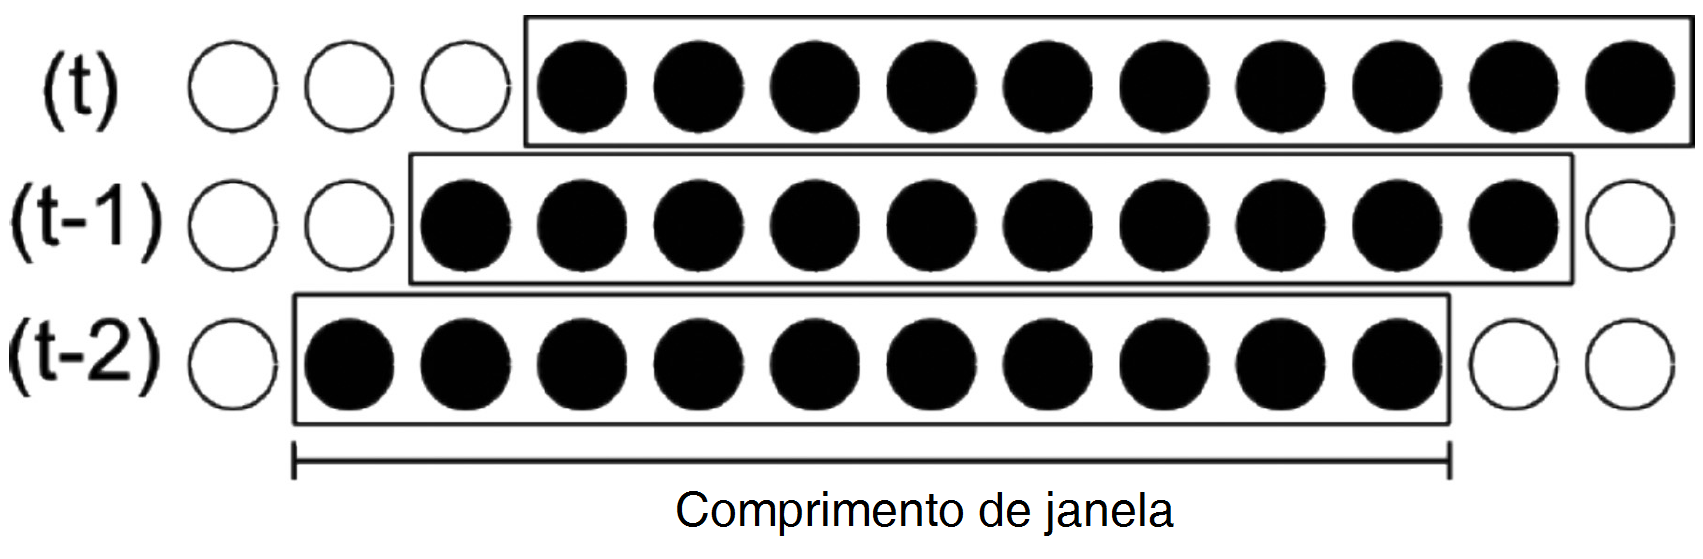
\includegraphics[width=\textwidth]{figures/slidingWindow}
                \caption{Modelo \emph{Sliding Window}}
                \label{Fig:slidingWindow}
        \end{subfigure}%
        \qquad %add desired spacing between images, e. g. ~, \quad, \qquad, \hfill etc.
          %(or a blank line to force the subfigure onto a new line)
        \begin{subfigure}[t]{0.4\textwidth}
                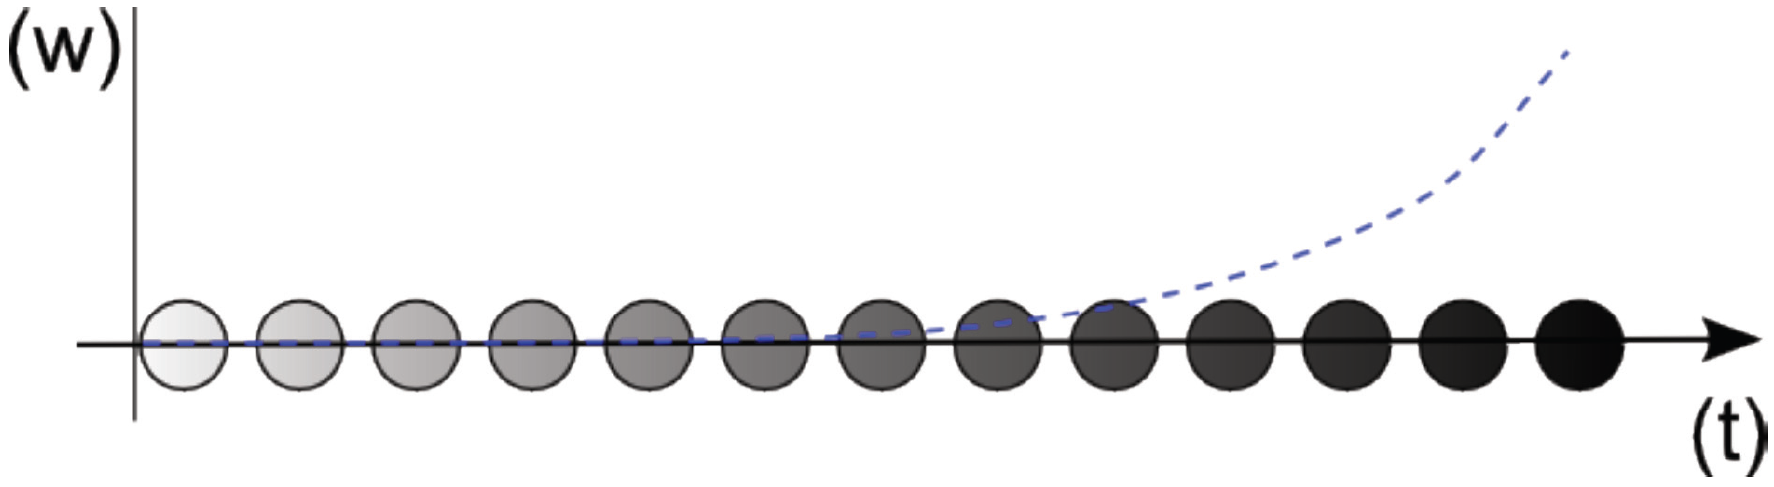
\includegraphics[width=\textwidth]{figures/dampedWindow}
                \caption{Modelo \emph{Damped Window}}
                \label{Fig:dampedWindow}
        \end{subfigure}
        \qquad %add desired spacing between images, e. g. ~, \quad, \qquad, \hfill etc.
        %(or a blank line to force the subfigure onto a new line)
        \begin{subfigure}[t]{0.4\textwidth}
        		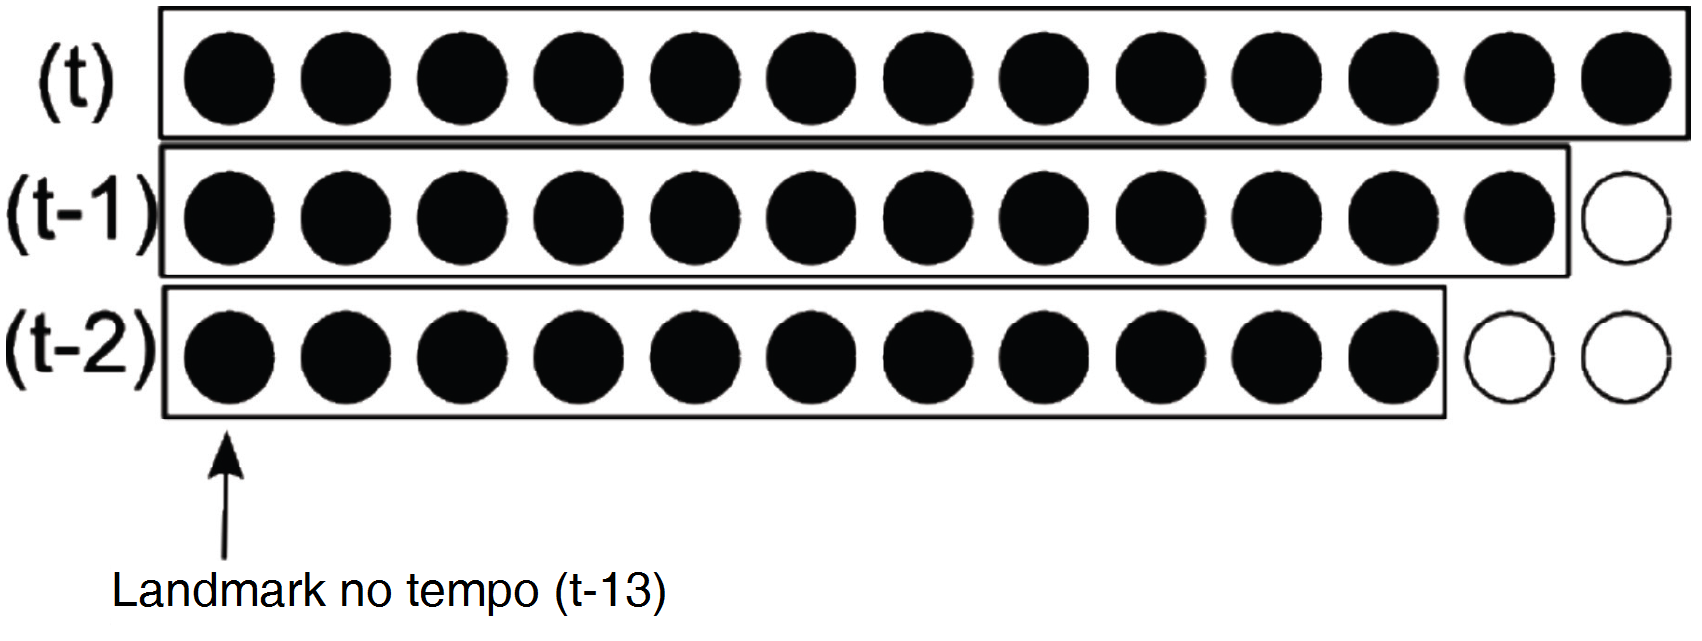
\includegraphics[width=\textwidth]{figures/landmarkWindow}
        		\caption{Modelo \emph{Landmark Window}}
        		\label{Fig:landmarkWindow}
        \end{subfigure}
        \caption{Exemplos ilustrativos de modelos de janela temporal \cite{Silva2013}}\label{Fig:modeloJanelas}
\end{figure}

Além das características mencionadas a respeito do volume de exemplos, há também um componente temporal inerente a aprendizado em FD. Os dados podem evoluir de acordo com o tempo e assim a distribuição do conjunto pode ser alterada. Deste modo, algoritmos que apenas sugerem adaptações para contornar as questões de volume de exemplos podem não ser soluções efetivas neste contexto. Algoritmos de aprendizado em FD devem ter foco claro na evolução dos dados \cite{aggarwal2007:Ch1}.

O uso de modelos de janela temporal podem auxiliar no tratamento de um dos aspectos da evolução dos exemplos do FD, por permitir uma avaliação de acordo com o tempo. No entanto, existem outros aspectos que podem ser explorados. A próxima seção fala sobre a difícil tarefa de identificação de desvios de conceito.